\section{Entwurf (Daniel)}\label{sec:entwurf}

\subsection{Entscheidungen}
\paragraph{UI-Bibliothek}
Im Unternehmen der beiden Autoren findet zeitgleich zu diesem Programmentwurf durch Kollegen ein Umbau der Web-Applikation hin zu React und Redux statt.
Um Synnergien zu nutzen und einen Transfer in die Praxis zu ermöglichen soll daher der Prototyp dieses Programmentwurfs auf den gleichen Technologien basieren.
Da das Ziel dieses Programmentwurfs eine Mobile Applikation ist, ergeben sich aus dieser Anforderung folgende Möglichkeiten:
\begin{itemize}
    \item (Progressive) Web App mittles React (Web)
    \item Hybride, native App mit React (Web) und PhoneGap
    \item Hybride, native App mit React Native
\end{itemize}

Aus diesen drei Alternativen ist React Native am nächsten an einer nativen Anwendung.
Im Gegensatz zu PhoneGap wird kein Webview in einer nativen Anwendung genutzt um eine Webapp darzustellen,
sonder es werden tatsächliche native UI-Elemente verwendet.
Dadurch fühlt sich die Anwendung nativer an.
Somit fällt hier die Entscheidung auf React Native.

\paragraph{Firebase-Bibliothek}
Da auch die Nutzung von Googles \textit{Firebase}-Plattform bereits als Anforderung gestellt ist,
gilt es auch hier eine Entscheidung zu treffen.

Google bietet zu Nutzung von Firebase verschiedene Bibliotheken an.
Dazu zählen eine Bibliothek für Web- bzw. JavaScript-Anwendungen und eine für Android und iOS-Anwendungen.
React Native ist als hybride App ein Teil von beidem.

Einerseits lässt sich die Web-Bibliothek relativ leicht einbinden.
Andereseits könnten sich Funktionalitäten wie Benachrichtigunen schwieriger gestalten.

Die Android-Bibliothek ist deutlich näher am Gerät, wodurch Funktionalitäten besser genutzt werden können.
Allerdings besteht hier der Aufwand die Funktionen nativ zu implementieren und React-Natives-JavaScript zu nutzen.

Das Beste aus diesen beiden Welten verbindet die Bibliothek \textit{React Native Firebase} \cite{invertas78:online}.
Sie stellt eine Zwischenschicht zur Verfügung um auf einfache Weise mit JavaScript-Code auf die native Firebase-Bibliothek zuzugreifen.
Die Bibliothek ist modular aufgebaut, sodass nur die benötigten Funktionalitäten zur Applikation hinzugefügt werden.
Das initiale Einrichten, sowie das hinzufügen bestimmter Module gestaltet sich etwas aufwändiger als die Nutzung der Web-Bibliothek.
Dieses Problem wird jedoch detaillierte Anleitungen kompensiert.

\paragraph{Firebase-Datenbank}
Firebase stellt zwei mögliche Datenbanken zur Verfügung \cite{ChooseaD77:online}.
Die \textit{Realtime Database} ist technisch gesehen ein großes (mehr oder weniger strukturiertes) JSON-Objekt.
Vor allem die Skalierung kann hierbei Problematisch werden.

Im Vergleich dazu werden die Daten im \textit{Cloud Firestore} geordneter dargestellt.
Eine Datenbank besteh aus Sammlungen, welche JSON-ähnliche Dokumente enthalten.
Dokumenten können wiederum Sammlungen enthalten.
Nachteilig am \textit{Cloud Firestore} ist, dass sich dieser noch im Beta-Stadium befindet.
Daher ist es möglich, dass diese Datenbank nicht völlig stabil ist.

Das Ergebnis dieses Programmentwurfs soll keine produktive Applikation, sondern ein Prototyp sein.
Außerdem ist es ein Teilziel neue Technologien anzuwenden.
Aus diesen Gründen wird in dieser Andwendung der \textit{Cloud Firestore} genutzt.

\subsection{Oberflächengestaltung}
Die Gestaltung der Oberflächen orientiert sich an den \textit{Material Design}-Richtlinien von Google.
Auf \cite{DesignMa49:online} werden Richtlinien und Konzepte vorgegeben,
welche Entscheidungen bei der Oberflächengestaltung übernehmen.
Die zudem vorhandene Übersicht an Komponenten lässt sich nutzen um passende Komponenten für einen Anwendungsfall zu finden.

Um erste Ideen für die Oberflächengestaltung zu sammeln,
werden mit Hilfe von dem Tool \textit{Fluid UI} \cite{FluidUIc8:online} sogenannte UI-Mockups erstellt.
Diese Mockups dienen als beispielhafte Vorlage für die spätere Entwicklung.


\begin{figure}[h]
    \centering
    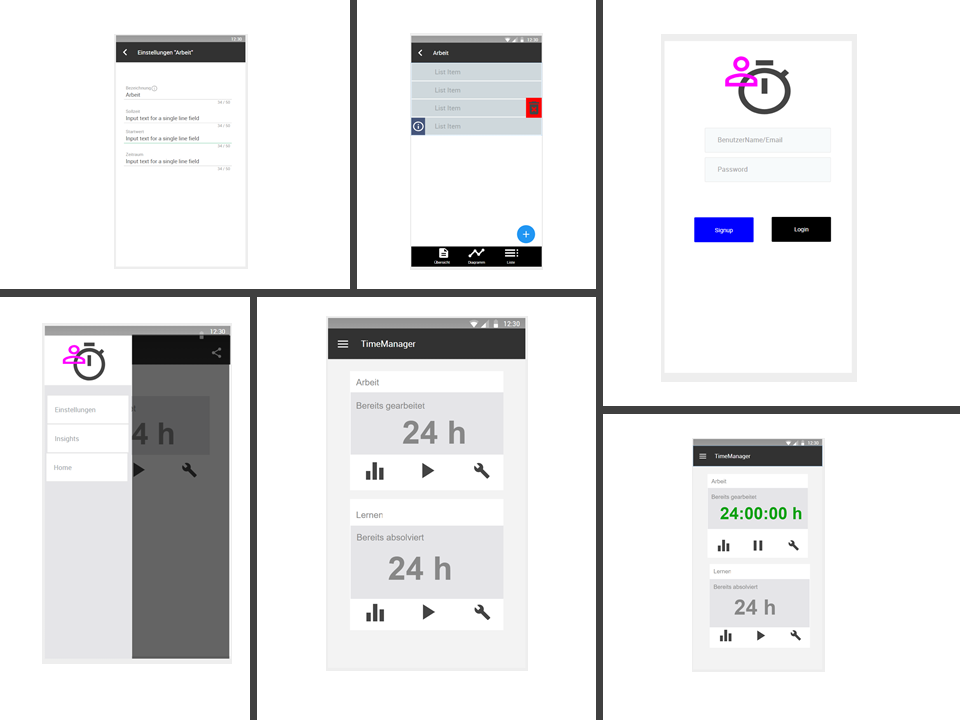
\includegraphics[width=\textwidth]{uiMocks/Mock}
    \caption{UI-Mockups der Anwendung}
\end{figure}



